\documentclass[10pt,x11names,table]{beamer}

\usetheme[progressbar=frametitle]{metropolis}
\usepackage{appendixnumberbeamer}
\usepackage{xcolor}

\usepackage{polyglossia}
\setmainlanguage{spanish}

\usepackage{listings}

\usepackage{booktabs}
\usepackage[scale=2]{ccicons}

\usepackage{pgfplots}
\usepgfplotslibrary{dateplot}

%ANIMACIONES
\usepackage{animate}
\usepackage{graphicx}
\usepackage[caption=false]{subfig}

\usepackage{xspace}

\newcommand*{\eg}{e.g.\@\xspace}
\newcommand*{\ie}{i.e.\@\xspace}

\let\oldquote\quote
\let\endoldquote\endquote
\renewenvironment{quote}[2][]
  {\if\relax\detokenize{#1}\relax
     \def\quoteauthor{#2}%
   \else
     \def\quoteauthor{#2~---~#1}%
   \fi
   \oldquote}
  {\par\nobreak\smallskip\hfill(\quoteauthor)%
   \endoldquote\addvspace{\bigskipamount}}
   
\usepackage{wrapfig}

\usepackage{subfig}
\usepackage{hyperref}
\usepackage{multicol}

\setbeamertemplate{bibliography item}[text]

\usepackage[font=small,skip=0pt, labelformat=empty]{caption}

\usepackage{dirtytalk}
\usepackage[acronym]{glossaries}
\makeglossaries

\newacronym{acgan}{ACGAN}{Auxiliary Classifier GAN}
\newacronym{ae}{AE}{Autoencoder}
\newacronym{ai}{AI}{Artificial Intelligence}
\newacronym{api}{API}{Application Programming Interface}
\newacronym{bert}{BERT}{Bidirectional Encoder Representations from Transformers}
\newacronym{brief}{BRIEF}{Binary Robust Independent Elementary Features}
\newacronym{brnn}{BRNN}{Bidirectional RNN}
\newacronym{bptt}{BPTT}{Backpropagation Through Time}
\newacronym{cbow}{CBOW}{Continous bag-of-words}
\newacronym{cnn}{CNN}{Convolutional Neural Network}
\newacronym{crnn}{CRNN}{Convolutional Recurrent Neural Network}
\newacronym{ddpm}{DDPM}{Denoising Diffusion Probabilistic Model}
\newacronym{ddim}{DDIM}{Denoising Diffusion Implicit Model}
\newacronym{diffit}{DiffiT}{Diffusion Vision Transformer}
\newacronym{dl}{DL}{Deep Learning}
\newacronym{dnn}{DNN}{Deep Neural Network}
\newacronym{dos}{DoS}{Denial of Service}
\newacronym{drnn}{DRNN}{Deep Recurrent Neural Network}
\newacronym{ecg}{ECG}{Electrocardiogram}
\newacronym{elmo}{ELMo}{Embedding from Language Model}
\newacronym{fast}{FAST}{Features from Accelerated Segment Test}
\newacronym{fid}{FID}{Fréchet Inception Distance}
\newacronym{foss}{FOSS}{Free and open-source software}
\newacronym{gan}{GAN}{Generative Adversarial Network}
\newacronym{glove}{GloVe}{Global Vectors for Word Representation}
\newacronym{gpu}{GPU}{Graphics Processing Unit}
\newacronym{gru}{GRU}{Gated Recurrent Unit}
\newacronym{ilsvrc}{ILSVRC}{ImageNet Large Scale Visual Recognition Challenge}
\newacronym{is}{IS}{Inception Score}
\newacronym{kid}{KID}{Kernel Inception Distance}
\newacronym{ldm}{LDM}{Latent Diffusion Model}
\newacronym{lstm}{LSTM}{Long Short-Term Memory}
\newacronym{mape}{MAPE}{Mean Absolute Perentage Error}
\newacronym{ml}{ML}{Machine Learning}
\newacronym{mlp}{MLP}{Multilayer Perceptron}
\newacronym{mmd}{MMD}{Maximum Mean Discrepancy}
\newacronym{mse}{MSE}{Mean Squared Error}
\newacronym{ner}{NER}{Named Entity Recognition}
\newacronym{nlg}{NLG}{Natural Language Generation}
\newacronym{nlp}{NLP}{Natural Language Processing}
\newacronym{nlu}{NLU}{Natural Language Understanding}
\newacronym{nn}{NN}{Neural Network}
\newacronym{ocr}{OCR}{Optical Character Recognition}
\newacronym{onnx}{ONNX}{Open Neural Network Exchange}
\newacronym{pmml}{PMML}{Predictive Model Markup Language}
\newacronym{relu}{ReLU}{Rectified Linear Unit}
\newacronym{rest}{REST}{Representational State Transfer}
\newacronym{rnn}{RNN}{Recurrent Neural Network}
\newacronym{sae}{SAE}{Stacked Autoencoder}
\newacronym{sift}{SIFT}{Scale-Invariant Feature Transform}
\newacronym{slam}{SLAM}{Simultaneous Localization and Mapping}
\newacronym{sru}{SRU}{Single Recurrent Unit}
\newacronym{surf}{SURF}{Speeded-Up Robust Features}
\newacronym{svm}{SVM}{Support Vector Machine}
\newacronym{vae}{VAE}{Variational Autoencoder}
\newacronym{vgg}{VGG}{Visual Geometry Group}
\newacronym{vit}{ViT}{Vision Transformer}
\newacronym{wsgi}{WSGI}{Web Server Gateway Interface}
\newacronym{xai}{XAI}{eXplainable Artificial Intelligence}
\newacronym{yolo}{YOLO}{You Only Look Once}
\newacronym{zsl}{ZSL}{Zero-shot Learning}
\subtitle{Métodos Generativos, curso 2024-2025}

\date{\today}
\author{Guillermo Iglesias, guillermo.iglesias@upm.es \newline
Jorge Dueñas Lerín, jorge.duenas.lerin@upm.es  \newline
Félix Fuentes Hurtado, felix.fuentes@upm.es}

\institute{Escuela Técnica Superior de Ingeniería de Sistemas Informáticos | UPM \newline
\hbox{} \newline \ccbysa \hspace{0.1pt} \ccNonCommercial}

%%%%%%%%%%%%%%%%%%%%%%%%%%%%%%%%%%%%%       
\title{Introducción a los métodos genetativos}

\begin{document}
\maketitle

\begin{frame}{Contenidos}
  \begin{enumerate}
      \item Introducción
      \item Auto-encoders (AEs)
      \item{Auto-encoders Variacionales (VAEs)}
      \item{Generative Adversarial Networks (GANs)}
      \item{Transformers}
      \item{Diffusion Models}
    \end{enumerate}
\end{frame}

\section{Introducción a los métodos generativos}

\begin{frame}{Paradigmas de aprendizaje y modelos}
Existen distintos paradigmas de aprendizaje y distintos tipos de modelos:
\begin{itemize}
    \item Aprendizaje supervisado vs. no supervisado
\end{itemize}

\begin{figure}
    \centering
    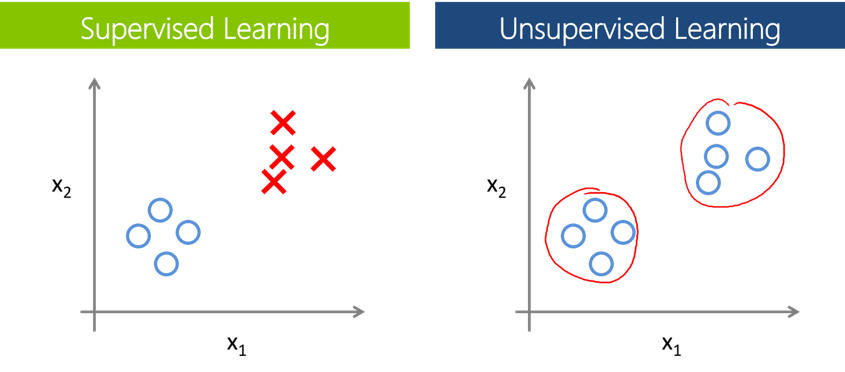
\includegraphics[width=0.7\textwidth]{Slides/figures/02_Metodos_Generativos/2.1. sup vs no sup.png}
\end{figure}
\end{frame}


\begin{frame}{Paradigmas de aprendizaje y modelos}
Existen distintos paradigmas de aprendizaje y distintos tipos de modelos:
\begin{itemize}
    \item Aprendizaje supervisado vs. no supervisado
    \item Modelos discriminativos vs. \textbf{generativos}
\end{itemize}

\begin{figure}
    \centering
    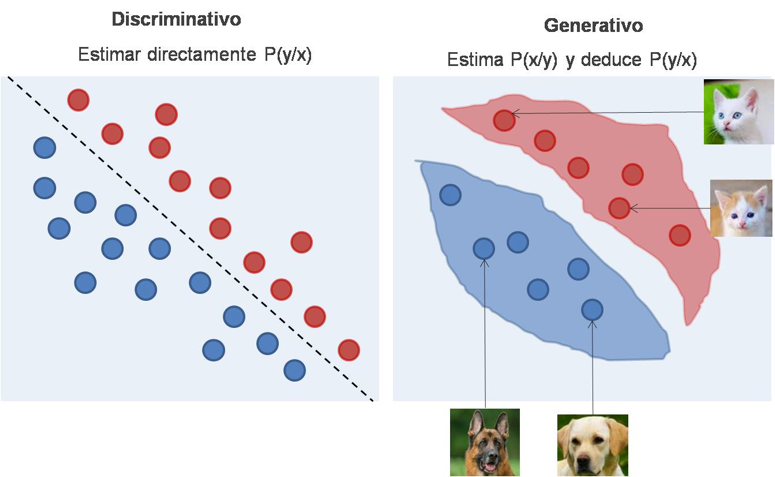
\includegraphics[width=0.7\textwidth]{Slides/figures/02_Metodos_Generativos/2.1. disc vs gen.png}
\end{figure}
\end{frame}


\begin{frame}{Paradigmas de aprendizaje y modelos}
\textbf{Tipos de modelos:}

\begin{itemize}
    \item \textbf{Discriminativos}: tratan de encontrar la dependencia entre los datos de entrada y los distintos tipos de clases
    \item \textbf{Generativos}: tratan de encontrar “cómo fueron generados” los datos teniendo en cuenta los distintos tipos de clases existentes
\end{itemize}

\begin{figure}
    \centering
    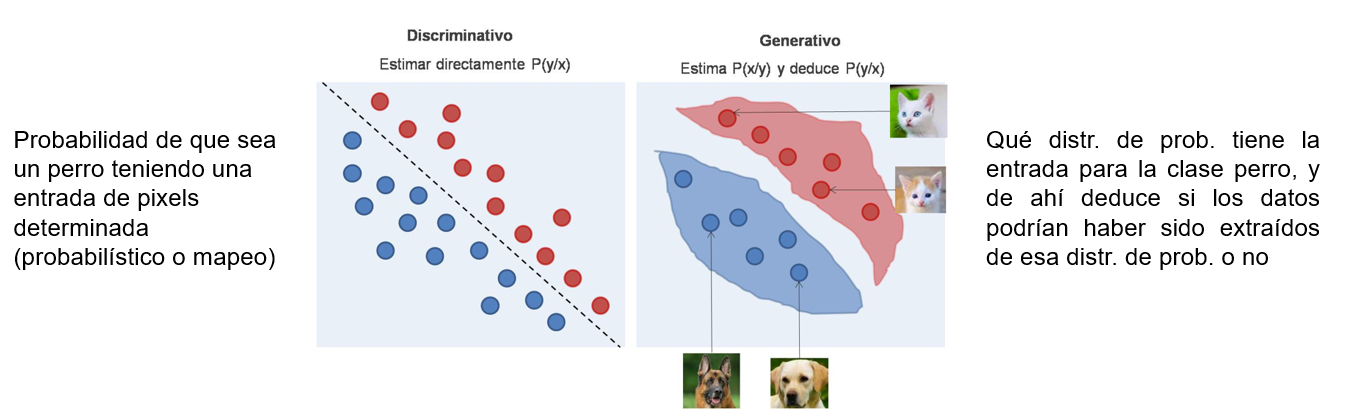
\includegraphics[width=\textwidth]{Slides/figures/02_Metodos_Generativos/2.1. disc gen.png}
\end{figure}
\end{frame}

\begin{frame}{Paradigmas de aprendizaje y modelos}
\textbf{Modelos discriminativos}

\begin{itemize}
    \item Son ampliamente utilizados en aplicaciones del mundo real debido a su eficacia en muchas tareas de aprendizaje supervisado.
    \item Se centran en aprender directamente la frontera de decisión entre clases o la función que mapea las entradas a las salidas.
    \item Generalmente son más rápidos en la fase de predicción una vez entrenados.
    \item Suelen tener un mejor desempeño en tareas de clasificación.
    \item Interpretabilidad variable: Algunos modelos (como árboles de decisión) son más interpretables, mientras que otros (como redes neuronales profundas) son menos transparentes.
    %\item Necesitan menos datos
    %\item Menor coste computacional
    %\item No son fáciles de interpretar
    %\item No tienen un buen desempeño en aprendizaje no supervisado
\end{itemize}

\end{frame}

\begin{frame}{Paradigmas de aprendizaje y modelos}
\textbf{Ejemplos de modelos discriminativos}

\begin{itemize}
    \item Regresión lineal/logística
    \item Árboles de decisión
    \item Support Vector Machines
    \item \textbf{Redes neuronales}
\end{itemize}

\end{frame}


\begin{frame}{Paradigmas de aprendizaje y modelos}
\textbf{Modelos generativos}

\begin{itemize}
    \item Además de aprender a diferenciar, también aprenden la estructura intrínseca de los datos.
    \item Modelan la distribución de probabilidad conjunta P(x,y) de las características x y las etiquetas y, o la distribución P(x) de los datos de entrada.
    \item Son útiles en aprendizaje no supervisado como clustering o reducción de dimensionalidad. También en detección de anomalías. 
    %\item Es más sencillo obtener una idea de qué caracteriza a una determinada clase. Modelos no basados en DL.
    \item Son más costosos computacionalmente.
\end{itemize}

\end{frame}

\begin{frame}{Paradigmas de aprendizaje y modelos}
\textbf{Ejemplos de modelos generativos}

\begin{itemize}
    \item Naive Bayes
    \item Máquinas de Boltzmann (RBM)
    \item Modelos de Markov (HMM)
    \item Gaussian Mixture Models (GMMs)
    \item Autoencoders variacionales (VAEs)
    \item Generative Adversarial Networks (GANs)
    \item Transformers
    \item Diffusion Models
\end{itemize}

\end{frame}


\begin{frame}{Modelos generativos tradicionales}

Antes de la época del Deep Learning ya existían modelos generativos, tanto basados en redes neuronales, como no basados en ellas.

Estos modelos generativos tradicionales han sido fundamentales en la modelización y generación de datos antes de la era del aprendizaje profundo.

Algunos de estos modelos basados en DL son:

\begin{itemize}
    \item Restricted Boltzmann Machines (RBMs)
    \item Hidden Markov Models (HMMs)
\end{itemize}

En cuanto a los no basados en redes neuronales, destacan los Gaussian Mixture Models (GMMs).

\end{frame}


\begin{frame}{Modelos generativos tradicionales}
\textbf{Naive Bayes:}
    \begin{itemize}
        \item Aprende la distribución conjunta de los datos y las etiquetas
        \item $P(C = \text{spam} \mid X = \text{"oferta"}, \text{"urgente"})$
        \item $P(C \mid X) = \frac{P(X \mid C) P(C)}{P(X)}$
    \end{itemize}
\end{frame}


\begin{frame}{Modelos generativos tradicionales}
\textbf{Restricted Boltzmann Machine (RBM):}
    \begin{itemize}
        \item Red neuronal restringida.
        \item Modelo de dos capas: capa visible y capa oculta.
        \item Emplea aprendizaje por divergencia contrastiva para entrenar.
    \end{itemize}
    
    \begin{columns}
    
        % Columna 1: Imagen
        \begin{column}{0.4\textwidth}
            \begin{figure}
            \centering
            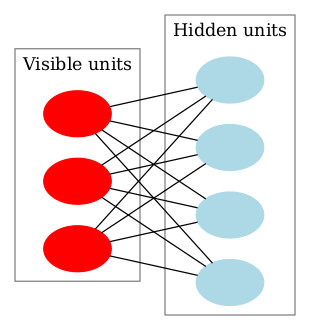
\includegraphics[width=\linewidth]{Slides/figures/02_Metodos_Generativos/Restricted_Boltzmann_machine.png}
            \caption{Wikipedia}
            \end{figure}
        \end{column}
        
        % Columna 2: Explicación en puntos
        \scriptsize{
        \begin{column}{0.6\textwidth}
            \begin{enumerate}
                \item \textbf{Paso hacia adelante}: Se ingresan datos a la RBM y la capa oculta se activa con esa información.
                \item \textbf{Reconstrucción}: A partir de la capa oculta, se intenta reconstruir los datos de entrada en la capa visible.
                \item \textbf{Comparación y ajuste}: Se compara la reconstrucción con los datos originales y se ajustan los pesos si hay diferencias.
                \item El proceso se repite varias veces para que la RBM mejore en la reconstrucción de los datos.
            \end{enumerate}
        \end{column}
        }
    \end{columns}
    
\end{frame}


\begin{frame}{Modelos generativos tradicionales}
    
\textbf{Hidden Markov Model (HMM):}
    \begin{itemize}
        \item Modela secuencias de datos como procesos de Markov ocultos.
        \item Ampliamente utilizado en procesamiento de señales y lenguaje natural.
        %\item Aplica el algoritmo de Viterbi para la decodificación de secuencias. JDL: No me da tiempo a mirar el algortimo para explicarlo por eso lo quito de la transparencia.
    \end{itemize}


    \begin{columns}
    
        % Columna 1: Imagen
        \begin{column}{0.4\textwidth}
            \begin{figure}
                \centering
                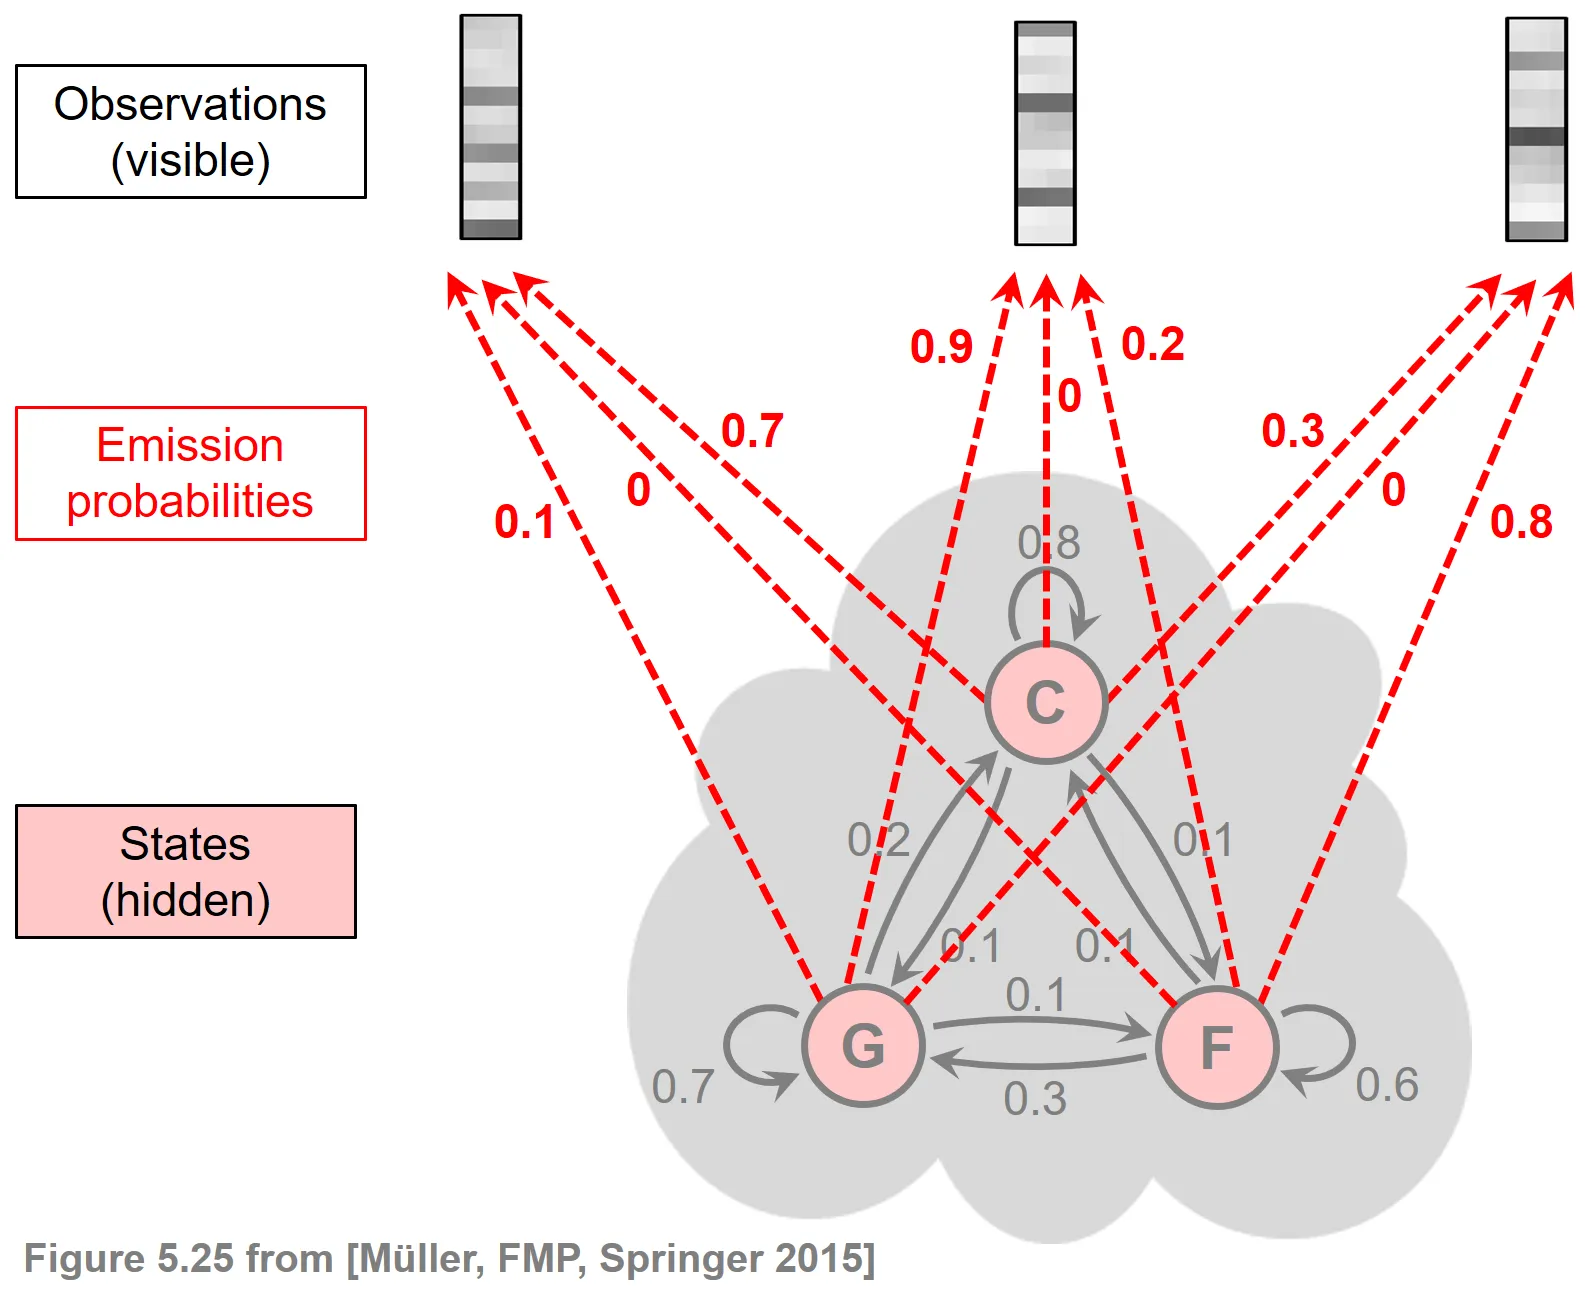
\includegraphics[width=1\linewidth]{Slides/figures/02_Metodos_Generativos/HMM.png}
                \caption{HMM}
                \label{fig:enter-label}
            \end{figure}
        \end{column}
        
        % Columna 2: Explicación en puntos
        \scriptsize{
        \begin{column}{0.6\textwidth}
            HMM sigue la premisa de que hay un conjunto de estados ocultos (no observables) que evolucionan con el tiempo de acuerdo a un proceso de Markov. Estos estados ocultos emiten las observaciones visibles.
            
            HMM modela la probabilidad conjunta de las observaciones X y los estados ocultos Y a lo largo del tiempo.
        \end{column}
        }
    \end{columns}


    

    
    
\end{frame}





\begin{frame}{Modelos generativos tradicionales}
\textbf{Gaussian Mixture Model (GMM):}
    \begin{itemize}
        \item Modela datos como mezcla de distribuciones gaussianas.
        \item Útil para modelar datos con múltiples modos o clusters.
        \item Emplea la expectativa-maximización (EM) para ajustar los parámetros.
        \item Se emplea tradicionalmente para \textit{\textbf{clustering}} de datos.
    \end{itemize}

    \begin{figure}
    \centering
    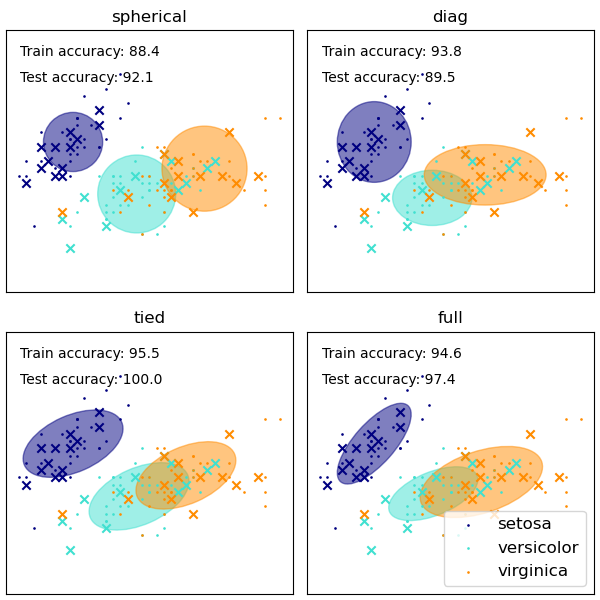
\includegraphics[width=0.4\textwidth]{Slides/figures/02_Metodos_Generativos/2.1. gmm cov.png}
    \caption{https://scikit-learn.org/stable/modules/mixture.html.}
    \end{figure}

\end{frame}


\begin{frame}{Contenidos}
  \begin{enumerate}
      \item Introducción
      \item Auto-encoders (AEs)
      \item{Auto-encoders Variacionales (VAEs)}
      \item{Generative Adversarial Networks (GANs)}
      \item{Transformers}
      \item{Diffusion Models}
    \end{enumerate}
\end{frame}


\iffalse

\begin{frame}{Gaussian Mixture Model (GMM)}
Los Gaussian Mixture Models (GMM) son modelos probabilísticos utilizados para describir conjuntos de datos como una combinación de múltiples distribuciones gaussianas.

\textbf{Combinación de Distribuciones Gaussianas:}
\begin{itemize}
    \item GMM asume que los datos son generados por la mezcla de varias distribuciones gaussianas.
    \item Cada componente gaussiano representa un "modo" o "cluster" en los datos.
    \item Los pesos indican la importancia relativa de cada componente en la mezcla.
\end{itemize}
\end{frame}


\begin{frame}{Gaussian Mixture Model (GMM)}
\textbf{Entrenamiento de GMM:}
\begin{itemize}
    \item Emplea el algoritmo de Expectation-Maximization (EM) para ajustar parámetros.
    \item \textbf{E-step}: Calcula las probabilidades de pertenencia a cada componente para cada dato.
    \item \textbf{M-step}: Ajusta los parámetros de las distribuciones gaussianas según las probabilidades.
\end{itemize}
\end{frame}


\begin{frame}{Gaussian Mixture Model (GMM)}
\textbf{Aplicaciones de GMM:}
\begin{itemize}
    \item \textbf{Agrupamiento de datos}: Identificar clusters en datos no etiquetados.
    \item \textbf{Modelado de datos complejos}: Modelar datos con estructuras multimodales.
    \item \textbf{Reducción de dimensione}s: GMMs pueden ser utilizados para reducir dimensiones al comprimir datos.
\end{itemize}
\end{frame}


\begin{frame}{Gaussian Mixture Model (GMM)}
\textbf{Ventajas:}
\begin{itemize}
    \item \textbf{Velocidad}: Es el algoritmo más \textbf{rápido} para aprender modelos de mixturas.
    \item \textbf{Agnóstico}: Dado que este algoritmo maximiza únicamente la verosimilitud, no sesgará las medias hacia cero ni sesgará los tamaños de los clústeres para tener estructuras específicas que podrían o no aplicarse.

\end{itemize}



\end{frame}




\begin{frame}{Gaussian Mixture Model (GMM)}
\textbf{Limitaciones:}
\begin{itemize}
    \item Requiere definir el número de componentes a priori.
    \item No siempre se ajusta bien a datos con formas complejas.
\end{itemize}
\end{frame}



\begin{frame}{Gaussian Mixture Model (GMM)}
Hace uso de la matriz de covarianza de los datos para ajustar la "forma" de las Gaussianas lo más posible:

\begin{figure}
    \centering
    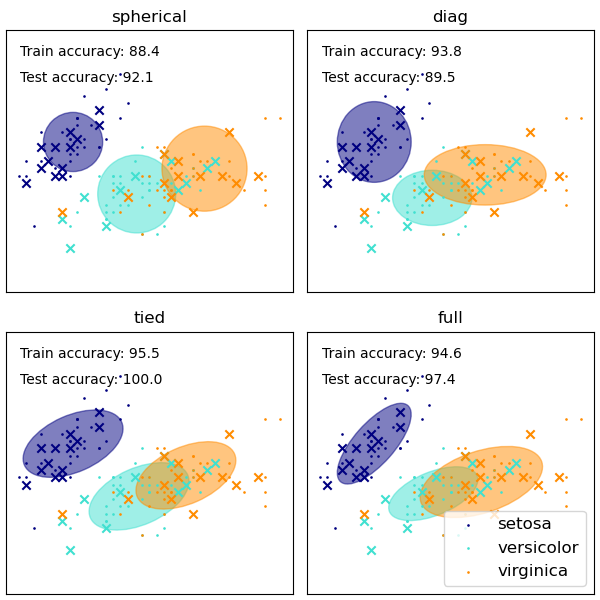
\includegraphics[width=0.4\textwidth]{Slides/figures/02_Metodos_Generativos/2.1. gmm cov.png}
    \caption{Imagen obtenida de https://scikit-learn.org/stable/modules/mixture.html.}
\end{figure}
\end{frame}

\fi

\begin{frame}{Recursos}
\begin{itemize}
    \item Diapositivas de Moodle
    \item Google Collaboratory
    \item Deep Learning Book (https://www.deeplearningbook.org/)
    \item https://www.pyimagesearch.com/blog
    \item https://machinelearningmastery.com/blog
\end{itemize}
\end{frame}


\appendix

% \begin{frame}[allowframebreaks]{Referencias}
%     \bibliography{references}
%     \bibliographystyle{abbrv}
% \end{frame}

\begin{frame}<presentation:0>{License}
    \begin{block}{Tema \texttt{slides-upm}. Puedes obtener sus fuentes en}
        \begin{center}\url{http://gitlab.com/blazaid/slides-upm}\end{center}
    \end{block}
  
    Tanto esta presentación como el tema están licenciados bajo \href{http://creativecommons.org/licenses/by-sa/4.0/}{Creative Commons
  Atribución-CompartirIgual 4.0 Internacional (CC BY-SA 4.0)}.
    \begin{center}\ccbysa\end{center}
\end{frame}

\end{document}
